% TODO More examples of the various different clause coverages
% Refine what is going on with minor clauses being the same.

\documentclass{beamer}
\usetheme{default}
\usepackage{tikz}
\usetikzlibrary{positioning}
\setbeamertemplate{footline}[page number]
\setbeamertemplate{navigation symbols}{}
\usepackage{hyperref}
\usepackage{listings}
\title{Software Testing  Lecture 5}
\author{Justin Pearson}
\date{2019}


%Lecture 4 stuff
\newcommand{\todo}[1]{{\tt ... #1 ... }}
\newcommand{\Reach}{\mathrm{Reach}}
\newcommand{\Path}{\mathrm{path}}

%Lecture 5 stuff
\newcommand{\predset}{{\cal P}}
\newcommand{\clauseset}{{\cal C}}
%Stolen from Stackexchange
%http://tex.stackexchange.com/questions/20609/strikeout-in-math-mode 
\newcommand\hcancel[2][red]{\setbox0=\hbox{$#2$}%
\rlap{\raisebox{.45\ht0}{\textcolor{#1}{\rule{\wd0}{1pt}}}}#2} 

\begin{document}
\lstset{language=C}

\begin{frame}
  \maketitle
\end{frame}

\begin{frame}{Covering Logical Expressions}
  \begin{itemize}
  \item Logic expressions show up in many situations
  \item Covering logical expressions has a long history, many are the
    covering criteria are mandated by the US FAA in safety critical
    software.
  \item Logical expressions can come from many sources:
    \begin{itemize}
    \item Decisions in programs
    \item Finite State Machines and statecharts 
    \item Requirements
    \end{itemize}
  \end{itemize}
  
\end{frame}
\begin{frame}{Interlude TCAS}
  \begin{itemize}
  \item Traffic collision avoidance system (TCAS)
  \end{itemize}
  Two aircraft flying towards each other, you have to decide which one
  goes up and which one goes down. From wikipedia:
  \begin{quote}
    The next step beyond identifying potential collisions is
    automatically negotiating a mutual avoidance manoeuver (currently,
    manoeuvers are restricted to changes in altitude and modification
    of climb/sink rates) between the two (or more) conflicting
    aircraft. These avoidance manoeuvers are communicated to the
    flight crew by a cockpit display and by synthesized voice
    instructions.
  \end{quote}
  
\end{frame}
\begin{frame}{TCAS}


  \begin{center}
        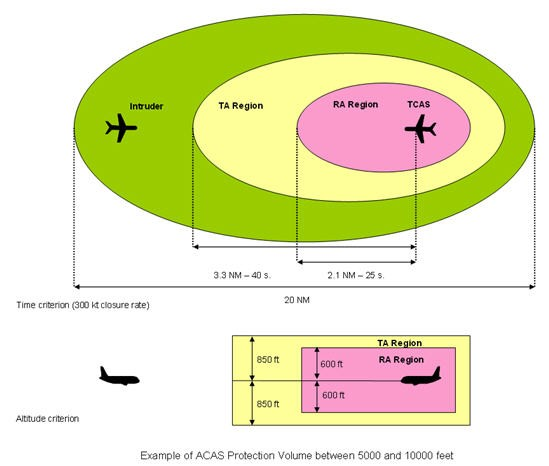
\includegraphics[height=2.5in,width=3.5in]{TCAS_Volume.jpg}
  \end{center}
There are rather a lot of complicated interacting logical requirements
that decide unambiguously how each aircraft should react.     
\end{frame}

\begin{frame}{Covering Logical Expressions}
  \begin{itemize}
  \item Typical balance in software testing:
    \begin{itemize}
    \item In theory, there are too many options to test everything.
    \item Find good coverage criteria that have a chance of covering
      useful cases.
    \item As usual there are no guarantees, but try to model cases that
      capture commonly occurring faults.
    \end{itemize}
  \end{itemize}  
\end{frame}


\begin{frame}[fragile]{Motivation}
  \begin{lstlisting}
    if ((x>0 && y>0) || z>0) 
        {do_something;} 
   else 
      {something_else;}
  \end{lstlisting}
Branch or edge coverage would only require one test case that executes
the two branches. Instead, you might want to test all the possibilities
of the logical expression.


  
\end{frame}
\begin{frame}[fragile]{Motivation}
\begin{tabular}{|l|l|l|l|}
  \hline 
  {\tt x>0} & {\tt y>0} & {\tt z>0} & \verb+((x>0 && y>0) || z>0)+ \\ 
  \hline
  T & T & T & T \\
  T & T & F & T \\
  T & F & T & T \\
  T & F & F & F \\
  F & T & T & T \\
  F & T & F & F \\
  F & F & T & T \\
  F & F & F & F \\
  \hline 
\end{tabular}

So a test corresponding to the line $TFT$ would require:
$x>0$, $y\leq 0$ and $z>0$. \newline You would have to find a test path with
these values.
\end{frame}
\begin{frame}[fragile]{Logical Connectives: Revisions?}
  \begin{tabular}{|l|l|l|}
    \hline
   $P$ & $Q$ & $P \land Q$, \verb+P && Q+ \\
    T  & T   & T \\
    T  & F   & F \\
    F  & T   & F \\
    F  & F   & F \\
    \hline
  \end{tabular}
  \begin{tabular}{|l|l|l|}
    \hline
   $P$ & $Q$ & $P \lor Q$, \verb+P || Q+ \\
    T  & T   & T \\
    T  & F   & T \\
    F  & T   & T \\
    F  & F   & F \\
    \hline
  \end{tabular}

  \begin{tabular}{|l|l|l|}
    \hline
   $P$ & $Q$ & $P \rightarrow Q$ \\
    T  & T   & T \\
    T  & F   & F \\
    F  & T   & T \\
    F  & F   & T \\
    \hline
  \end{tabular}
  \begin{tabular}{|l|l|l|}
    \hline
   $P$ & $Q$ & $P \leftrightarrow Q$ \\
    T  & T   & T \\
    T  & F   & F \\
    F  & T   & F \\
    F  & F   & T \\
    \hline
  \end{tabular}
  \begin{tabular}{|l|l|l|}
    \hline
   $P$ & $\neg P$, \verb+!P+ \\
    T  & F \\
    F  & T \\
    \hline
  \end{tabular}

  \begin{tabular}{|l|l|l|}
    \hline
   $P$ & $Q$ & $P \oplus Q$ Exclusive Or \\
    T  & T   & F \\
    T  & F   & T \\
    F  & T   & T \\
    F  & F   & F \\
    \hline
  \end{tabular}
\end{frame}

\begin{frame}[fragile]{Predicates and Clauses}
  \begin{itemize}
  \item A {\em predicate} is an expression that evaluates to true or
    false.
   \item A predicate may contain:
     \begin{itemize}
     \item Boolean variables.
     \item Expressions evaluating to  Boolean variables that contain
       comparison operation {\tt >, < , ==, >=, != , <=}
     \item  Boolean function calls.
     \end{itemize}
   \item Internal structure is created by logical operators (see
     previous slide)
   \item A clause is a predicate with no logical operators.
     \begin{itemize}
     \item $P \land Q$ is a predicate
     \item \verb+x>0+ is a clause. 
     \end{itemize}
  \end{itemize}
\end{frame}

\begin{frame}{Testing and Covering Predicates}
  \begin{itemize}
  \item Reduce the artefact to a set of predicates
  \item State covering criteria in terms of predicates and clauses.  
  \end{itemize}
  \begin{itemize}
  \item $\predset$ - the set of predicates.
  \item $p$ is a single predicate in $\predset$.
  \item $\clauseset$ - set of clauses in $\predset$.
  \item $\clauseset_p$ - set of clauses in predicate $p$.
   \item $c$ is a single clause in $\clauseset$.
  \end{itemize}
\end{frame}
\begin{frame}{Predicate Coverage}

Very simple and very blunt.
  \begin{itemize}
  \item {\em Predicate Coverage (PC)}: For each $p$ in $\predset$, the {\it test requirements}
   include that $p$ evaluates to true and $p$ evaluates to false. 
  \end{itemize}

\end{frame}
\begin{frame}[fragile]{Predicate Coverage}

  \begin{lstlisting}
    if (x>0 || y>0) 
      {do_something;} 
    else
      {something_else;}
    if (z>0) 
       {foo;}
    else
       {bar;}
  \end{lstlisting}
The predicates are \verb+x>0 || y>0+ and \verb+z>0+. So we have 4 {\it test
requirements}. So test case inputs could be $x=3\land y=-10$,
$x=-3\land y=-10$, $z=20$ and $z=-120$.
\end{frame}
\begin{frame}{Clause Coverage}
  \begin{itemize}
  \item Not every clause is exercised. 
  \end{itemize}
So we get a new coverage criterion.
\begin{itemize}
\item {\em Clause Coverage (CC)} - For each clause $c$ in
  $\clauseset$, we have a test requirement that $c$ evaluates to true
  and $c$ evaluates to false.
\end{itemize}
\end{frame}
\begin{frame}[fragile]{Clause Coverage}
  \begin{lstlisting}
    if (x>0 || y>0) 
      {do_something;} 
    else
      {something_else;}
    if (z>0) 
       {foo;}
    else
       {bar;}
  \end{lstlisting}
The clause are \verb+x>0+, \verb+y>0+ and  \verb+z>0+.  So we have 6
{\it test requirements}. 
\end{frame}
\begin{frame}{Example}
\[
((a<b) \lor D) \land (m \geq n)
\]
\begin{itemize}
\item Predicate true: $a=5$, $b=10$, $D$ is true, $m=1$ and $n=1$.
\item $((5<10) \lor T) \land (1 \geq 1) = (T \lor T )\land T$
\end{itemize}

\begin{itemize}
\item Predicate false: $a=10$, $b=5$, $D$ is false, $m=1$ and $n=1$.
\item $((5<10) \lor F) \land (1 \geq 1) = (T \lor T )\land T$
\item $(F \lor F) \land T = F$.
\end{itemize}

\end{frame}
\begin{frame}{Clause Coverage}
\[
((a<b) \lor D) \land (m \geq n)
\]
Test requirements 
\begin{itemize}
\item $a<b$ is true: $a=5$, $b=10$.
\item $a<b$ is false: $a=10$, $b=5$.
\item $D$ is true and $D$ is false.
\item $m\geq n$ is true: $m=1$, $n=1$.
\item $m\geq n$ is false: $m=1$, $n=2$.
\end{itemize}
We can do this with two test cases:
\begin{itemize}
\item $a=5, b=10$, $D$ is true, $m=1$ and $n=1$. 
\item $a=10$,$b=5$, $D$ is false, $m=1$ and $n=2$.
\end{itemize}
  
\end{frame}

\begin{frame}[fragile]{Problems with Predicate and Clause Coverage} 
  \begin{itemize}
  \item Predicate coverage does not fully exercise all the clauses,
    especially in the presence of short circuit evaluation:
    \begin{center}
      \begin{verbatim}
         P && Q
      \end{verbatim}
    \end{center}
  \item If \verb+P+ is false then \verb+Q+ is never
    evaluated\footnote{It is a bit more complicated than this.} in C++.
  \end{itemize}
  
\end{frame}
\begin{frame}[fragile]{Problems with Predicate and Clause Coverage} 
  \begin{itemize}
  \item Clause coverage does not imply predicate coverage.
  \item We can satisfy clause coverage without causing the predicate
    to be  true and false.
    \[
     (P \lor Q) \land R
    \]
    \item Clauses $P$, $Q$ and $R$. Thus, we have 6 {\it test requirements} $P=T$,$P=F$,
    $Q=T$,$Q=F$, $R=T$ and $R=F$.
  \item $(P=F \lor Q=F)    \land R=T$ evaluates to false.
  \item $(P=T \lor Q=T)    \land R=F$ evaluates to false.
  \item All {\it test requirements} covered.  So we need something better,
    all possibilities?
  \end{itemize}  
\end{frame}
\begin{frame}{Combinatorial Coverage}
  \begin{itemize}
  \item {\em Combinatorial Coverage} For each $p$ in $\predset$, the
    test requirement includes that each clause in $C_p$ evaluates to
    each possible combination of truth values.
  \item That really means test all rows in the truth table. 

  \end{itemize}
\end{frame}
\begin{frame}{Combinatorial Coverage}
  \begin{itemize}
    \item Simple, clean, neat, and comprehensive.
  \item But, it can be quite expensive $2^N$ tests for $N$ clauses. 
  \item Lots of suggestions in the literature, but the general idea is
    simple:
    \begin{itemize}
    \item Test each clause {\em independently} from the other clauses.
    \end{itemize}
  \item You have to work out what exactly does independent mean. The
    book uses the concept {\em ``making clauses active''}.
  \end{itemize}
\end{frame}
\begin{frame}{Active Clauses}
  \begin{itemize}
  \item The major weakness of clause coverage is that the values do
    not always make a difference.
  \item We really want the test results of a clause to be a
    determining factor in the truth or falsehood of the predicate.
  \end{itemize}
  
\end{frame}
\begin{frame}{Determination}
  \begin{itemize}
  \item {\em Major clause}  is the clause under consideration.
  \item {\em Minor clause}  are the rest of the clauses.
  \item Let $c_i$ be the major clause in a predicate $p$. Then
    $c_i$ determines $p$ if and only if the value of the remaining
    minor clauses are such that changing the value of $C_i$ changes
    the value of $p$. 
  \end{itemize}
  
\end{frame}
\begin{frame}{Determining Predicates}

  \begin{itemize}
  \item $P = A \lor B$.
    \begin{itemize}
    \item Major clause A, and minor clause B. If $B=F$ then A determines $P$. 
    \item Major clause B, and minor clause A. If $A=F$ then B determines $P$.
    \end{itemize}
  \item $Q = A \land B$.
    \begin{itemize}
    \item if $B=F$ then $Q$ is always false. 
    \item If $B=T$ then $A$ determines $p$.
    \end{itemize}
  \end{itemize}
  \end{frame}


\begin{frame}{Determining Predicates}
    
  \begin{itemize}
  \item For a determining clause you have to take into account the
    assignments of the minor clauses.

  \item Basic idea is: for each clause you want assignments to the minor
clauses so that your clause becomes a determining clause.
\item It becomes more complicated, when you consider how the different
  {\it test requirements} overlap.
  \end{itemize} 
\end{frame}
%Slide 16.
\begin{frame}{Active Clause Coverage}
  \begin{itemize}
  \item {\em Active Clause Coverage (ACC):} For each predicate $p$ in
    $\predset$ and each major clause, choose values for the  minor
    clauses so that the major clause determines $p$. The {\it test
    requirements} contain  requirements so  that the major clause
    evaluates to true and the major clause evaluates to false.
  \end{itemize}

  
\end{frame}
\begin{frame}{Active Clause Coverage}
\[
 P = A \lor B 
\]
  \begin{itemize}
  \item $A$ as the major clause.
    \begin{itemize}
    \item $A=T$, $B=F$
    \item $A=F$, $B=F$.
    \end{itemize}
  \item $B$ as the major clause.
    \begin{itemize}
    \item $B=T$, $A=F$
    \item $\hcancel{B=F, A=F}$.
    \end{itemize}
  \end{itemize}
 There is a source of {\em ambiguity}: Do the minor clauses have to
 have the same values when the major clause is true and false?
\end{frame}
\begin{frame}{Resolving the Ambiguity}
\[
P = A \lor (B \land C)
\]
Major clause $A$:
\begin{itemize}
\item $A=T$, $B=F$, $C=T$
\item $A=F$, $B=F$, $C=F$
\end{itemize}
Do we allow different assignments to the minor clauses?

Three possible criteria:
\begin{itemize}
\item Minor clauses {\em do not } need to be the same.
\item Minor clauses {\em do} need to be the same.
\item Minor clauses {\em force predicate} to become both true and false.
\end{itemize}
  
\end{frame}
\begin{frame}{General Active Clause Coverage}

{\em General Active Clause Coverage}: For each predicate $p$ in
$\predset$ and each major clause in $C_p$, choose minor clauses so
that it determines $p$.{\it Test requirements} include that the major
clause evaluates to true and false. The values of the minor clauses do
{\em not} need to be the same.

This is the most general definition. 
\end{frame}
\begin{frame}{General Active Clause Coverage}
General active clause coverage does not imply predicate coverage.

\[
P = A \leftrightarrow B
\]
\begin{itemize}
\item Major clause $A$
  \begin{itemize}
  \item $A=T$, $B=F$ , $P = A\leftrightarrow B = F$.
  \item $A=F$, $B=T$.  $P = A\leftrightarrow B = F$.
  \end{itemize}
\item Major Clause $B$
  \begin{itemize}
  \item $B=T$, $A=F$, $P = A\leftrightarrow B = F$.
  \item $B=F$, $A=T$, $P = A\leftrightarrow B = F$.
  \end{itemize}
\end{itemize}
We have general active clause coverage, but the predicate always
evaluates to false. We really want clauses to cause predicates to
evaluate to both true and false.
  
\end{frame}
\begin{frame}{Restricted Active Clause Coverage}
  \begin{itemize}
  \item {\em Restricted Active Clause Coverage:} For each predicate
    and each major clause in each predicate, choose values of minor
    clauses so that the major determines the predicate.{\it Test
    requirements} include each major clause evaluates to true and
    false. The values chosen for the minor clauses {\bf must be the
      same}.
  \item Been used in aviation software. 
  \item No logical reason for the values of the minor clauses to be
    the same. 
  \item We still haven't solved the problem of the predicate
    evaluating to both true and false.
  \end{itemize}
  
\end{frame}
\begin{frame}{Correlated Active Clause Coverage}
  \begin{itemize}
  \item {\em Correlated Active Clause Coverage:} For each predicate
    and each major clause in each predicate, choose values of minor
    clauses so that the major clause determines the predicate. {\it Test
    requirements} include each major clause evaluates to true and
    false. The values of the minor clauses must be chosen such that
    the predicate evaluates to true and false.
  \end{itemize}
\end{frame}
\begin{frame}{Correlated Active Clause Coverage}
  \[
   A \land (B \lor C)
  \]
  \begin{itemize}
  \item Major Clause $A$.
    \begin{itemize}
    \item $A=T$, $B=T$, $C=T$, $A\land (B\lor C)=T$
    \item $A=F$, $B=T$, $C=F$, $A\land (B\lor C)=F$
    \end{itemize}
  \end{itemize}
\end{frame}

\begin{frame}{Making clauses determine a predicate}
  \begin{itemize}
  \item Finding values for minor clauses is easy for simple
    predicates.
  \item A trick help with more complicated predicates.
  \item $P_{c=T}$, replace every occurrence of $c$ by $T$.
  \item $P_{c=F}$, replace every occurrence of $c$ by $F$.
  \item Solving $P_{c=T} \oplus P_{c=F} = T$ gives you the
    values of the minor clauses for the major clause $c$ to determine
    the predicate.
  \end{itemize}
Remember that $A\oplus B$ is equivalent to $(A\lor B) \land \neg (A
\land B)$. 
\end{frame}
\begin{frame}{Making clauses determine a predicate}
  \begin{itemize}
  \item $P=A\lor B$, Major clause $A$.
    \begin{itemize}
    \item $P_A = P_{A=T} \oplus P_{A=F} = (T \lor B) \oplus (F
      \lor B)$ which gives $T \oplus B = \neg B$. 
    \item So $B$ must be false.
    \end{itemize}
    \item $P=A\land B$, Major clause $A$.
    \item $P_A = P_{A=T} \oplus P_{A=F} = (T \land B) \oplus (F
      \land B)$ which gives $B \oplus F =  B$. 
    \item So $B$ must be true.
  \end{itemize}
\end{frame}
\begin{frame}{Making clauses determine a predicate}
  \begin{itemize}
  \item $P=A\lor (B\land C)$, Major clause $A$.
    \begin{itemize}
    \item $P_{A=T} \oplus P_{A=F} = (T \lor (B\land C)) \oplus
      (F 
      \lor (B\land C))$ which gives $T\oplus (B\land C) = \neg (B
      \land C) = \neg B \lor \neg C$.
    \item So $B=F$ and $C=T$ is a solution.
    \item $A \lor (F \land T) = A \lor F$. 
    \end{itemize}

  \end{itemize}
\end{frame}
\begin{frame}{Determination is not always possible}
  Consider $p = (a\land b) \lor  (a\land \neg b)$ 
  \begin{itemize}
  \item $p_{b=T} \oplus p_{b=F} = (a\land T) \lor (a\land \neg T) \oplus
    (a\land F) \lor (a\land \neg F)$
  \item $=(a \lor F) \oplus (F \lor a)$
  \item $=a \oplus a$ which is always false. 
  \end{itemize}
If you think about this, then it should not be too surprising.  In
this case $b$ is redundant.
\end{frame}
\begin{frame}{Logic Coverage Summary}
  \begin{itemize}
  \item Combinatorial coverage gives too many test cases.
  \item Predicate coverage is too blunt.
  \item Clause coverage has to be refined to force the predicate to
    evaluate to both true and false.
  \item We want the test case to do some work, so we use correlated
    active clause coverage. The are lots of different variations, but
    it is important to remember major, minor clauses determining a
    predicate, requiring the predicate to be true or false. The
    variations are then on requirements on how the clauses overlap.
  \end{itemize}
  Think about infeasible   test requirements: $X>0 \land X<0$.
\end{frame}
\begin{frame}{Common Themes}
  \begin{itemize}
  \item Define coverage, even in a finite case there are too many
    cases to consider.
  \item Look for restrictions, but look for restrictions that find
    test cases that actually do some work.
  \item Try to maximise the overlapping test cases for each
    requirement in order to minimise the number of test cases needed.
  \item As usual there are no (or very few) theoretical guarantees.
  \item In some domains standards are mandated. 
  \end{itemize}
\end{frame}
\end{document}

%%% Local Variables:
%%% mode: latex
%%% TeX-master: t
%%% End:
